%!TEX root = ..\..\dissertation.tex
\chapter{Research Approach}\label{chp:Approach}
A central aspect of this thesis is the creation of new knowledge on manufacturing system platforms with both theoretical uses and practical applications.
With the limited existing research in the field and continuing difficulties in developing and utilising manufacturing system platforms in companies, new theories, concepts, methods, models, and tools contributing to the state-of-the-art are needed.
In particular, the steps and tools required in going from realising platforms, modules, and changeable manufacturing are needed, to identifying, developing, and documenting these for future use.
Thus, considering the above and the state-of-the-art presented in \cref{chp:Introduction}, the overall objective of this thesis can be formulated as below.
\begin{objective}
Create and apply methods and tools for identifying, developing, and documenting manufacturing system platforms through commonality and standardisation of assets
%, thereby supporting manufacturers in creating changeable manufacturing systems
\end{objective}
The focus on creation of new knowledge and its application in companies calls for a research approach centred around this.
It should be an approach that can be employed for research on both manufacturing systems, products, and systems engineering as a whole, in order to account for future co-development and the necessary alignment between these departments in a company.
In the following sections, the applied design science research approach is outlined, the industrial case presented, and finally the research objective is framed by individual research questions and sub-questions. 
% The interplay of design science research with these theories and concepts forms the contextual foundation of this research, as illustrated on \cref{fig:contextFound}.
% \begin{figure}[tb]
%   \centering
%   \missingfigure[figwidth=\textwidth]{contextual foundation}
%  \caption{Contextual foundation for this research, showing the main theories and works on which it is based, as well as their relation.}\label{fig:contextFound}
% \end{figure}

%!TEX root = ..\..\dissertation.tex
\section{Design Science Research}\label{sec:DSR}
%Intro?
\posscite{10.2307/25148625} framework for design science in information systems (IS) research emphasises creation of new knowledge, and its application in real world scenarios.
It is a conceptual framework for conducting research on information systems by combining design science and behavioural science, \ie{} the search for utility (effective artefacts) and the search for truth (justified theory), respectively~\parencite{10.2307/25148625}.
An effective \gls{glos:artefact} is, for the purposes of the research framework, a concrete entity addressing and facilitating understanding of problems.
\textcite{10.2307/25148625} describes four type of \gls{glos:artefact}s: ``\emph{constructs} (vocabulary and symbols), \emph{models} (abstractions and representations), \emph{methods} (algorithms and practices), and \emph{instantiations} (implemented and prototype systems)''.
In the design science framework, development of artefacts is initiated by problems or needs in an environment.
Using applicable knowledge, \eg{} theories, frameworks, or existing artefacts, new artefacts are built or designed and consistently evaluated in order to justify their existence and continued development.
Finished and justified artefacts are applied and tested in an appropriate environment, and subsequently added to a knowledge base along with any newly acquired experiences and developed theories.

\textcite{Hevner2007TheTC} introduced the notion of design science research cycles to the original research framework, resulting in the iteration shown on \cref{fig:ISRframework}.
\begin{figure}[tb]
  \centering
  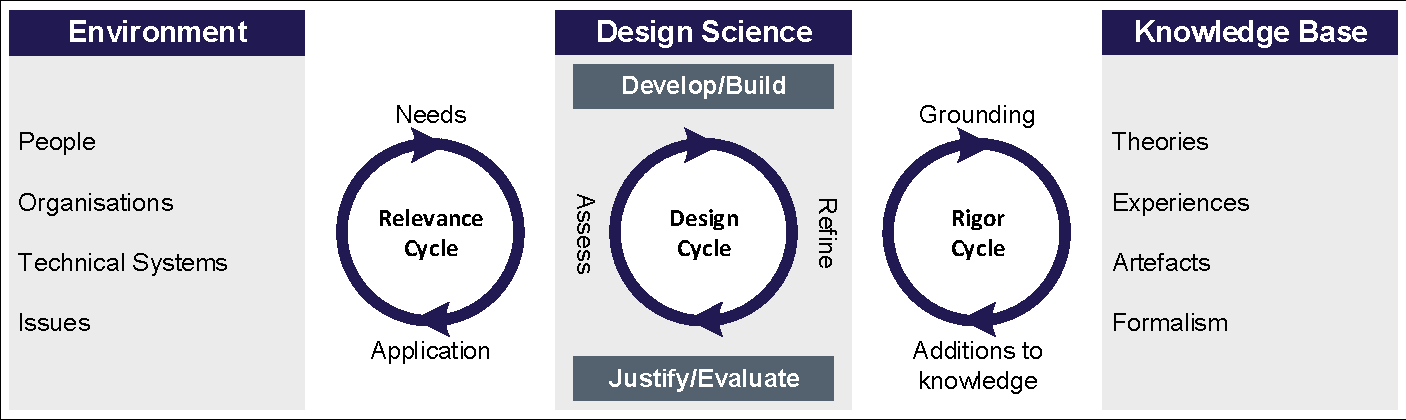
\includegraphics[width=\textwidth, trim=2 2 2 2, clip]{mainmatter/approach/figures/ISRframework.pdf}
  \caption{\posscite{Hevner2007TheTC} information systems framework and design science research cycles.}\label{fig:ISRframework}
\end{figure}
The \emph{relevance cycle} provides a context for application of the design science research results, along with a specification of the requirements and determination of acceptance criteria for evaluating the outcome of the research.
It connects the design activities to the overall context for the research project.
Needs are defined in the environment, \ie{} the problem space, and provide an input to be processed by design science activities.
Every artefact developed based on the needs from the environment is applied within the context of the environment, and field tested to determine the artefact's utility.
Through the \emph{rigor cycle}, the design activities are founded in scientific theories, experiences, and existing artefacts in a knowledge base while newly developed artefacts, theories, experiences, and potential extensions to already existing entries are fed back to the knowledge base.
Central to the design activities and project is the \emph{design cycle} itself.
In this cycle, the two core design activities of building (developing) and evaluating (justifying) are carried out iteratively.
Artefacts are built, evaluated, and refined until a satisfactory result is achieved.
The requirements upon which the evaluation is based are input from the relevance cycle, while the evaluation, development, and refinement methods are all pulled from the rigor cycle.
As \textcite{Hevner2007TheTC} put it, ``it is important to understand the dependencies of the design cycle on the other two cycles while appreciating its relative independence during the actual execution of research.''

The four types of artefacts are all highly relevant to the development of manufacturing system platforms.
Construct artefacts, defined as vocabulary and symbols, is essentially the language and manner in which problems and solutions are communicated and defined.
While the platforms are discussed increasingly frequently in research and within companies, there are still several individual understandings and opinions of \eg{} what constitutes a platform, how a module is defined, what a manufacturing process or manufacturing system is~\parencite{SorensenMCPC2017,SorensenAPMS2018}.
Developing constructs, \eg{} in the shape of employee handbooks, classification schemes, and modelling formalisms, makes communication during platform projects easier and helps avoid misunderstandings.
They also function as templates and forms for documenting platforms and their development.
Model \gls{glos:artefact}s use the vocabulary defined in constructs to represent the problem, solution, environment, and the link between them.
They are tools to be used during platform development, \eg{} to represent the functional structure of a platform in development, highlight how requirements are realised in the modules of a platform, or ways of representing entire manufacturing systems and their characteristics.
Abstracting various aspects of platforms in this manner is useful to manage the complexity of the development process.

Method \gls{glos:artefact}s are processes or procedures guiding problem solving and decision-making.
An informal method can be a simple text, describing how a manufacturing process is carried out, or how a model is built and used.
Method artefacts can also be formal mathematical algorithms, \eg{} providing a measure of the commonality between two systems, or a recommendation on which platforms to develop.
Instantiation \gls{glos:artefact}s are artefacts implemented to solve a problem in an environment.
This can, for instance, be the actual decision of selecting a potential platform based on an algorithm applied to a classification coding scheme.
An instantiation artefact may also be an implemented manufacturing system platform.
Examples of these are few and far between, but remain critical to the continued research within the field as a way to demonstrate the feasibility of both the platforms and the artefacts, theories, and experiences that helped create them.

The design science in information systems research framework outlined above is an appropriate fit for research on manufacturing system platforms since it is, as discussed in \cref{ssec:pPlatforms}, a field of relative immaturity.
Thus, the notion of employing knowledge bases aligns with, as others have suggested, gaining inspiration and applying concepts from other fields of research, thereby contributing to the knowledge base on manufacturing system platforms with new experiences and artefacts.
Further, with its focus on application of artefacts to solve real-world problems within a defined environment context, it lends itself well to case-studies, where new tools and methods are developed, or existing tools and methods are applied in a new context.
Another reason for choosing this framework, is that it is both proactive and reactive with respect to technology~\parencite{10.2307/25148625}.
Proactive, in the sense that design science focuses on creating and evaluating technology and artefacts, allowing the industry to address their needs through the artefacts.
Reactive, as behavioural science focuses on developing and justifying theories related to the implementation and use of technology and artefacts.
Research on platforms should be developed and evaluated in a collaborative context between academia and the industry.
%!TEX root = ..\..\dissertation.tex
\section{Industrial Case}
% \todo[inline]{Case 25/06}
This \PhD{} project is affiliated with, and partly funded by, the national research initiative, Manufacturing Academy of Denmark (MADE), specifically the first iteration, MADE SPIR (Strategic Platform for Innovation and Research) in work package 2 (WP2) on modular production platforms\footnote{\url{http://made.dk/spir}}.
MADE is essentially a collaboration of Danish universities, companies, and technology institutes working towards addressing issues in the Danish manufacturing industry and keeping Danish manufacturers competitive on a global scale.

The primary collaborator for this \PhD{} project is a large, Danish-founded manufacturer of discrete products for both domestic and industrial applications.
Currently, the company employs over 19,000 people, distributed across several factories and sales offices in more than 50 countries, with their main headquarters and the majority of their factories located in Denmark, as summarised in~\cref{tab:caseOverview}.
Every year, hundreds of manufacturing systems produce millions of complete products, packed and ready for sale to private or industrial customers, as well as components, sub-assemblies, and custom solutions to industrial partners.
With in-house final assembly and production of components and sub-assemblies, the company is essentially horizontally integrated.
Many of the case company's manufacturing systems are largely contracted designs by a variety of system integrators, while some systems include manufacturing equipment designed entirely in-house.
Thereby resulting in a high variety of the manufacturing systems themselves, with manufacturing equipment from a wide range of suppliers and system integrators.

Recently, the case company has been seeing a high demand for rapid introduction of new products, an upswing in product variety, and an accelerated time-to-market, along with a continuous pressure to increase productivity and lower costs.
This has lead to a need for an accelerated product and production development process, which in turn lead to the realisation that the case company must introduce the capability to efficiently accommodate change through standardisation---thus, \gls{glos:changeability} through platforms.

Stakeholders within the case company have been working towards increased modularity and standardisation in products and production for several years. 
Development and support truly picked up speed in 2014 with participation in MADE SPIR, thereby acquiring additional resources in the shape of collaboration with researchers from Aalborg University.
The first large platform co-development project was initiated in 2015, intended to kick-start development of a product platform and a manufacturing system platform for a specific set of products and related production systems.
It involved designers, developers, experts, and stakeholders from both product and production as well as \PhD{} and \MSc{} students from two Danish universities.
Focus for this project was essentially to design the first iteration of a platform-based product and production architecture, intended to be the foundation of any future new products and manufacturing systems within the scoped product and production segment.
Additional details on platform projects with the primary collaborator, the challenges that appeared, and recommendations on how to address these have been outlined in \parencite{SorensenAPMS2018}.

As a result of an increased focus on platforms and standardisation, various initiatives related to big data have been initiated within the company, including the formation of a new department whose task is to gather and standardise production data.
Data on manufacturing systems has proven crucial in the continued development of platforms within the case company, and the required data has historically been inadequate or completely missing.
A seemingly simple question such as ``how many manufacturing systems do we have?'' has turned out difficult to answer, due to varying definitions and opinions on what exactly constitutes a manufacturing system.
Outside the immediate intended benefits of utilising platforms, \eg{} accelerated time-to-market, increased process robustness, and simplified variety management, a number of other related benefits are expected as an indirect result of platform development, as outlined in the concluding remarks, \cref{chp:Conclusions}.

For the purposes of this \PhD{} project, a segment of the case company's production has been selected to act as primary production context.
The selected production segment is the assembly of a mechatronic sub-assembly, covering a wide range of production processes and automation degrees ranging from manual through semi-automated to fully automated.
This production segment consists of 20 manufacturing systems, producing 24 product architectures, covering both high-runner products with an annual volume over 2 million, and specialised products numbering 5,000 annually.
Size, mass, shape, and functionality also vary greatly across product architectures.
\cref{tab:caseOverview}~summarises the case company and the segment of their production covered in this research.
Characteristics below the second line refer only to the production segment covered in this study.
\begin{table}[tb]
  \centering
  \caption[Overview of the industrial case.]
  {Overview of the industrial case.
  The first four rows refer to the company as a whole, while the remaining rows refer only to the selected production segment.}\label{tab:caseOverview}
  \small
  \begin{tabular}{ll}
    \toprule%
    Characteristic & Value\\
    \midrule
    Company Size & Large \(>19,000\) employees\\
    Industry & Private and industrial mechatronic products\\
    Manufacturing Paradigm & Mass production\\
    Manufacturing System Paradigm & Dedicated manufacturing\\
    \midrule
    Production Context & Mechatronic sub-assembly\\
    Location & 4 factories in 4 different countries\\
    Production Volume & 5k--2mil annually\\
    Product Variety & 24 product architectures\\
    Production Variety & 20 production architectures\\
    Production Planning & Make-to-stock\\
    Automation & Manual, semi-automated and fully-automated\\
    Cycle time & 9\si{\second}--90\si{\second}\\
    \bottomrule%
  \end{tabular}
\end{table}

\section{Research Questions}\label{sec:RQ}
In order to further frame this thesis and elaborate on the research objective listed in the beginning of this chapter, three overall research questions have been formulated.
Each research question is addressed through one or more sub-questions from six research tasks, documented in the six appended papers.
While the overall research approach is the design science research framework described in \cref{sec:DSR}, a number of other methods have also been used for the individual appended papers.
For each sub-question, the paper it originates from is listed along with the selected research methods.
\begin{resq}\label{resq1}
  How can manufacturing system platforms be developed and documented using well-known concepts from software systems engineering and architecture, and which challenges arise during this process? 
  \begin{enumerate}[leftmargin=3em, label=RQ\arabic{resq}.\arabic*]
    \item How can production platforms be developed and documented with the aid of concepts and constructs from the field of software systems architecture? (Paper~\ref{paper:MCPC2017}; multi case study)
    \item Which challenges arise during manufacturing system platform development, and how can these be addressed? (Paper~\ref{paper:MCPC2017}; multi case study)
  \end{enumerate}
\end{resq}
\begin{resq}\label{resq2}
  How can commonality in processes across manufacturing systems be classified and used to identify candidates for manufacturing system platforms?
  \begin{enumerate}[leftmargin=3em, label=RQ\arabic{resq}.\arabic*]
    \item How can processes during production of discrete products be classified independently of the means facilitating the process? (Paper~\ref{paper:CMS2018}; literature review, iterative search and consolidation)
    \item What are the essential aspects of manufacturing systems that must be captured in order to classify them? (Paper~\ref{paper:clsfCoding}; design science research, classification, analysis, development and refinement of artefacts and knowledge)
    \item What is the best form/structure of a coding scheme that captures and classifies essential manufacturing system aspects/characteristics? (Paper~\ref{paper:clsfCoding}; design science research, classification, analysis, development and refinement of artefacts and knowledge)
    \item How can a production system classification coding scheme be used to identify candidates for a manufacturing system platform? (Paper~\ref{paper:APMS2019}; design science research, single case study, application in environment)
  \end{enumerate}
\end{resq}
\begin{resq}\label{resq3}
  How can manufacturing system platforms be developed in a brownfield approach taking into account a manufacturer's existing production landscape and which challenges arise over time as platform development progresses?
  \begin{enumerate}[leftmargin=3em, label=RQ\arabic{resq}.\arabic*]
    \item Which challenges do mature manufacturers face over time, when developing manufacturing system platforms? (Paper~\ref{paper:APMS2018}; design science research, evolving case study)
    \item What steps should a manufacturer take to develop platforms of standardised assets based on existing manufacturing systems and environments? (Paper~\ref{paper:CMS2019}; conceptual research, evolving case study)
  \end{enumerate}
\end{resq}